\documentclass[11pt]{article}

% Review version: includes line numbers and page numbers (8 pages max)
\usepackage[review]{acl}

% Standard package includes
\usepackage{times}
\usepackage{latexsym}
\usepackage{amsmath}

% For proper rendering and hyphenation of words containing Latin characters (including in bib files)
\usepackage[T1]{fontenc}

% This assumes your files are encoded as UTF8
\usepackage[utf8]{inputenc}

% This is not strictly necessary, and may be commented out,
% but it will improve the layout of the manuscript,
% and will typically save some space.
\usepackage{microtype}

% This is also not strictly necessary, and may be commented out.
% However, it will improve the aesthetics of text in
% the typewriter font.
\usepackage{inconsolata}

%Including images in your LaTeX document requires adding
%additional package(s)
\usepackage{graphicx}

% For tables
\usepackage{booktabs}

% For figures and diagrams
\usepackage{tikz}
\usetikzlibrary{shapes,arrows,positioning}

\title{Multi-Agent LLM-Based Test Generation: A Comparative Study of Single, Collaborative, and Competitive Approaches}

\author{Anonymous Author(s) \\
  Affiliation / Address line 1 \\
  Affiliation / Address line 2 \\
  Affiliation / Address line 3 \\
  \texttt{email@domain}}

\begin{document}
\maketitle
\begin{abstract}
Automated test generation remains a critical challenge in software engineering. This paper presents a comparative evaluation of three multi-agent approaches for generating test cases using Large Language Models (LLMs): single-agent generation, collaborative multi-agent generation with specialized roles, and competitive adversarial generation. We implement and evaluate these approaches on a curated subset of 19 functions from the HumanEval dataset, measuring both code coverage (line and branch) and test diversity (syntactic patterns, unique assertions). Our experimental results reveal distinct trade-offs: single-agent generation achieves the highest line coverage (22.9\%) and diversity score (0.598), while competitive generation produces the most unique test patterns (20) and highest branch coverage (11.1\%). Collaborative generation, despite employing three specialized agents, achieves lower coverage (9.7\% line, 0\% branch), suggesting that current deduplication strategies may be overly aggressive. These findings contribute to understanding how multi-agent LLM systems can be effectively applied to automated test generation and highlight important considerations for balancing coverage and diversity in generated test suites.
\end{abstract}

\section{Introduction}

Automated test generation is a fundamental problem in software engineering, with significant implications for software quality, development velocity, and maintenance costs. Traditional approaches to test generation, including search-based testing \cite{McMinn2004}, symbolic execution \cite{Cadar2008}, and fuzzing \cite{Manes2019}, have shown promise but often require domain-specific expertise and may struggle with complex code structures or modern programming paradigms.

Recent advances in Large Language Models (LLMs) have demonstrated remarkable capabilities in code generation and understanding \cite{Chen2021}. These models can generate syntactically correct code, understand natural language specifications, and reason about program behavior. This has naturally led to interest in applying LLMs to automated test generation, where the model's ability to understand code semantics and generate diverse test scenarios could complement traditional approaches.

However, the effectiveness of LLM-based test generation depends critically on how the generation process is structured. Single-agent approaches, where one LLM instance generates all tests, may miss edge cases or lack diversity. Multi-agent systems, where multiple LLM instances collaborate or compete, offer the potential for more comprehensive test coverage through specialized roles or adversarial dynamics.

\subsection{Research Questions}

This paper addresses the following research questions:

\begin{enumerate}
\item How do single-agent, collaborative multi-agent, and competitive multi-agent LLM approaches compare in terms of test coverage and diversity?
\item What are the trade-offs between code coverage (line and branch) and test diversity across these approaches?
\item How effective are specialized agent roles in collaborative test generation?
\end{enumerate}

\subsection{Contributions}

Our contributions are threefold:

\begin{itemize}
\item We present three distinct multi-agent frameworks for LLM-based test generation: single-agent baseline, collaborative generation with specialized roles, and competitive adversarial generation.
\item We provide a comparative evaluation on a curated subset of the HumanEval dataset, measuring both coverage and diversity metrics.
\item We analyze the trade-offs between coverage and diversity, identifying strengths and limitations of each approach.
\end{itemize}

\section{Background}

\subsection{Automated Test Generation}

Automated test generation has been an active area of research for decades. Search-based testing techniques \cite{McMinn2004} use evolutionary algorithms to evolve test inputs that maximize coverage metrics. Symbolic execution \cite{Cadar2008} explores program paths symbolically to generate inputs that reach specific code locations. Fuzzing techniques \cite{Manes2019} generate random or mutation-based inputs to discover bugs. While effective, these approaches often require significant manual configuration and may struggle with complex control flow or modern language features.

\subsection{LLM-Based Code Generation}

Large Language Models have shown remarkable success in code-related tasks. Codex \cite{Chen2021} demonstrated that LLMs can generate functional code from natural language descriptions. Subsequent work has explored code completion, bug fixing, and code explanation. The application of LLMs to test generation is a natural extension, leveraging the model's understanding of code semantics and ability to generate diverse scenarios.

\subsection{Multi-Agent Systems}

Multi-agent systems have been explored in various domains, including collaborative problem-solving and competitive optimization \cite{Stone2007}. In software testing, the concept of using multiple agents with different perspectives or strategies has been explored in mutation testing and fuzzing. Collaborative agents can complement each other's strengths, while competitive agents can drive exploration through adversarial dynamics. Recent work has shown that multi-agent LLM systems can improve performance on complex tasks through specialization and coordination \cite{Wang2023}.

\subsection{Test Quality Metrics}

Test quality is typically measured along multiple dimensions. Code coverage metrics, including line coverage and branch coverage, measure the proportion of code exercised by tests. Diversity metrics assess how different tests are from each other, which can indicate whether tests explore distinct scenarios. Both metrics are important: high coverage ensures thoroughness, while high diversity reduces redundancy and increases the likelihood of finding different types of bugs.

\section{Methodology}

\subsection{Architecture Overview}

Our system implements three distinct test generation approaches, all built on a common LLM abstraction layer. Figure~\ref{fig:architecture} illustrates the overall architecture.

\begin{figure*}[t]
\centering
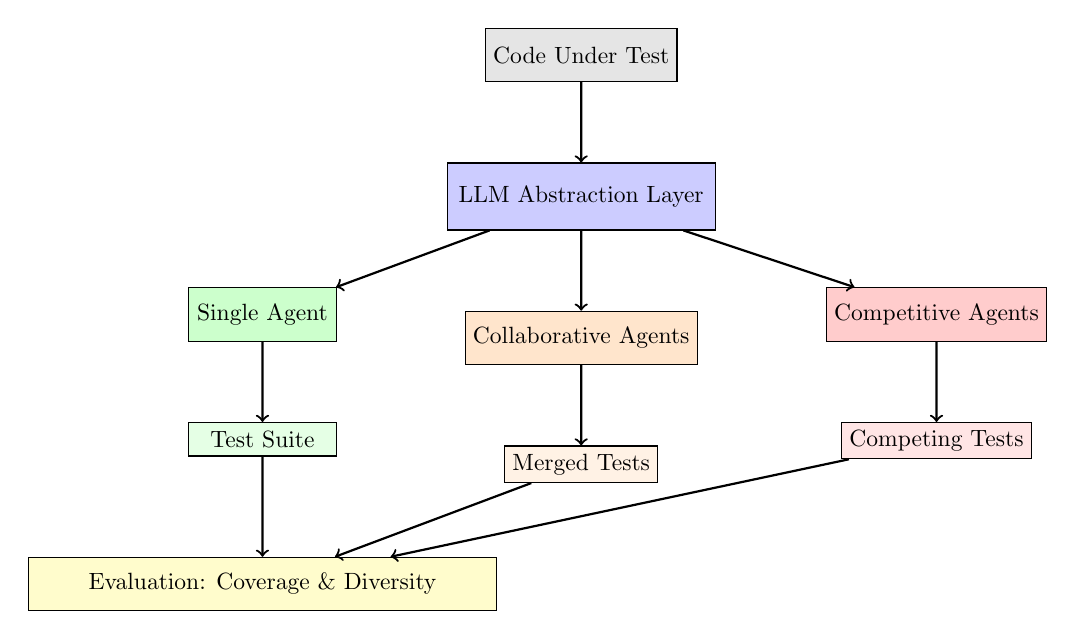
\begin{tikzpicture}[node distance=1.2cm, auto, scale=0.85, transform shape]
    % CUT Input
    \node [rectangle, draw, fill=gray!20, minimum width=2.5cm, minimum height=0.8cm] (cut) {Code Under Test};
    
    % LLM Layer
    \node [rectangle, draw, fill=blue!20, minimum width=4cm, minimum height=1cm, below=of cut] (llm) {LLM Abstraction Layer};
    
    % Single Agent
    \node [rectangle, draw, fill=green!20, minimum width=2.2cm, minimum height=0.8cm, below left=of llm, xshift=-0.8cm] (single) {Single Agent};
    \node [rectangle, draw, fill=green!10, minimum width=2.2cm, minimum height=0.5cm, below=of single] (single_out) {Test Suite};
    
    % Collaborative
    \node [rectangle, draw, fill=orange!20, minimum width=2.2cm, minimum height=0.8cm, below=of llm] (collab) {Collaborative Agents};
    \node [rectangle, draw, fill=orange!10, minimum width=2.2cm, minimum height=0.5cm, below=of collab] (collab_out) {Merged Tests};
    
    % Competitive
    \node [rectangle, draw, fill=red!20, minimum width=2.2cm, minimum height=0.8cm, below right=of llm, xshift=0.8cm] (comp) {Competitive Agents};
    \node [rectangle, draw, fill=red!10, minimum width=2.2cm, minimum height=0.5cm, below=of comp] (comp_out) {Competing Tests};
    
    % Evaluation
    \node [rectangle, draw, fill=yellow!20, minimum width=7cm, minimum height=0.8cm, below=of single_out, yshift=-0.3cm] (eval) {Evaluation: Coverage \& Diversity};
    
    % Arrows
    \draw [->, thick] (cut) -- (llm);
    \draw [->, thick] (llm) -- (single);
    \draw [->, thick] (llm) -- (collab);
    \draw [->, thick] (llm) -- (comp);
    \draw [->, thick] (single) -- (single_out);
    \draw [->, thick] (collab) -- (collab_out);
    \draw [->, thick] (comp) -- (comp_out);
    \draw [->, thick] (single_out) -- (eval);
    \draw [->, thick] (collab_out) -- (eval);
    \draw [->, thick] (comp_out) -- (eval);
\end{tikzpicture}
\caption{System architecture showing three generation modes: single-agent, collaborative, and competitive, all built on a common LLM abstraction layer.}
\label{fig:architecture}
\end{figure*}


\subsection{LLM Abstraction Layer}

The system provides a unified interface to LLM providers, supporting both local models (via Ollama) and online APIs (OpenAI). The abstraction layer handles model configuration, error handling, and fallback mechanisms. Configuration is managed through environment variables, allowing flexible deployment across different environments. The implementation supports configurable temperature, maximum tokens, and timeout settings, enabling fine-tuning of generation behavior.

The abstraction layer defaults to local Ollama but automatically falls back to OpenAI if local models are unavailable. Error handling covers timeouts, rate limits, and quota exhaustion.

\subsection{Single-Agent Generation}

Single-agent generation serves as our baseline approach. The process follows these steps:

\begin{enumerate}
\item Load the Code Under Test (CUT) module dynamically using Python's \texttt{importlib}.
\item Extract source code using Python's \texttt{inspect} module.
\item Format a prompt template with the CUT code and generation parameters.
\item Call the LLM with the formatted prompt.
\item Extract Python code from the LLM response, handling markdown code blocks.
\item Validate the generated code using AST parsing to ensure syntax correctness.
\item Check for test functions (functions starting with \texttt{test\_}) and assertions.
\item Save the validated test code to a timestamped output directory.
\end{enumerate}

The prompt template instructs the LLM to generate pytest-compatible test functions covering normal cases, edge cases, and error scenarios. The template emphasizes proper import statements, descriptive test names, and comprehensive assertions.

The single-agent approach includes quality validation checking for assertions, proper imports, and function calls. If quality falls below 60\%, the system retries with adjusted temperature settings.

\subsection{Collaborative Generation}

Collaborative generation employs multiple specialized agents, each with a distinct testing perspective. Our implementation uses three agents:

\begin{itemize}
\item \textbf{Edge Case Agent}: Focuses on boundary conditions, extreme values, and exception scenarios.
\item \textbf{Boundary Value Agent}: Emphasizes boundary value analysis and off-by-one errors.
\item \textbf{Integration Agent}: Targets integration scenarios and real-world usage patterns.
\end{itemize}

Each agent receives a role-specific prompt template that guides its generation strategy. The agents generate tests independently, and the results are merged through a deduplication process:

\begin{enumerate}
\item Extract test functions from each agent's response using AST parsing.
\item Deduplicate by function name (exact match).
\item Deduplicate by code similarity using normalized string comparison.
\item Combine unique test functions into a single test file.
\item Validate the merged code for syntax and test function presence.
\end{enumerate}

The deduplication strategy aims to preserve diversity while removing exact duplicates. However, our results suggest this may be overly aggressive, potentially removing tests that are similar but test different scenarios.

\subsection{Competitive Generation}

Competitive generation implements an adversarial workflow where two agents compete:

\begin{enumerate}
\item \textbf{Agent 1} generates an initial test suite using standard test generation.
\item \textbf{Agent 2} reviews Agent 1's tests and generates competing tests based on a competition mode.
\item Tests from both agents are merged and deduplicated.
\end{enumerate}

We implement three competition modes:

\begin{itemize}
\item \textbf{Adversarial}: Agent 2 performs gap analysis to find bugs and edge cases Agent 1 missed.
\item \textbf{Diversity}: Agent 2 generates tests that maximize diversity from Agent 1's tests.
\item \textbf{Coverage}: Agent 2 targets uncovered code paths and branches.
\end{itemize}

Our experiments use the adversarial mode, where Agent 2's prompt explicitly instructs it to identify gaps in Agent 1's coverage and generate complementary tests.

\subsection{Evaluation Metrics}

We evaluate generated tests along two dimensions:

\subsubsection{Coverage Metrics}

We measure both line coverage and branch coverage using Python's \texttt{coverage.py} tool. Coverage is measured by running the generated tests with pytest and analyzing which lines and branches of the CUT module are executed. Line coverage measures the proportion of executable lines covered, while branch coverage measures the proportion of conditional branches (if/else, loops) exercised.

Coverage measurement instruments the CUT module during test execution, tracking executed lines and taken branches to generate detailed reports with summary statistics and per-function breakdowns.

\subsubsection{Diversity Metrics}

We calculate syntactic diversity using AST-based analysis:

\begin{itemize}
\item \textbf{Diversity Score}: Calculated as $1 - \text{average\_pairwise\_similarity}$, where similarity is measured using Jaccard similarity on AST token sets. Higher scores indicate more diverse tests.
\item \textbf{Unique AST Patterns}: Count of distinct AST structures across all tests.
\item \textbf{Unique Assertions}: Count of distinct assertion patterns.
\item \textbf{Unique Calls}: Count of distinct function calls made in tests.
\end{itemize}

The diversity score ranges from 0 (all tests identical) to 1 (completely different tests). We use syntactic diversity as our primary diversity metric, as it captures structural differences in test code that may indicate different testing strategies.

The diversity calculation parses test functions into ASTs, extracts structural patterns, and computes pairwise similarities to capture differences in test structure, assertion patterns, and function call diversity.

\section{Experimental Setup}

\subsection{Dataset}

We evaluate our approaches on a curated subset of 19 functions from the HumanEval dataset \cite{Chen2021}. HumanEval is a benchmark for evaluating code generation capabilities, containing 164 programming problems with function signatures, docstrings, and test cases. We selected functions covering diverse categories:

\begin{itemize}
\item \textbf{Math/Statistics}: \texttt{truncate\_number}, \texttt{mean\_absolute\_deviation}, \texttt{greatest\_common\_divisor}, \texttt{sum\_product}, \texttt{rescale\_to\_unit}, \texttt{factorize}
\item \textbf{List Operations}: \texttt{has\_close\_elements}, \texttt{below\_zero}, \texttt{intersperse}, \texttt{rolling\_max}, \texttt{sort\_numbers}, \texttt{find\_closest\_elements}, \texttt{remove\_duplicates}
\item \textbf{String Operations}: \texttt{parse\_nested\_parens}, \texttt{filter\_by\_substring}, \texttt{make\_palindrome}, \texttt{string\_xor}, \texttt{count\_distinct\_characters}, \texttt{flip\_case}
\end{itemize}

Each function includes provenance information (task ID, entry point) linking it to the original HumanEval dataset. All functions are standalone and require only Python standard library imports.

\subsection{Experimental Configuration}

Our experiments follow this configuration:

\begin{itemize}
\item \textbf{Single-agent}: Generate 10 test functions per run.
\item \textbf{Collaborative}: 3 agents, each generating 10 test functions (target: 30 total before deduplication).
\item \textbf{Competitive}: 2 agents, adversarial mode, each generating 10 test functions (target: 20 total before deduplication).
\end{itemize}

All experiments use the same LLM configuration: Ollama with the \texttt{qwen2.5-coder:14b-instruct} model, with fallback to OpenAI if local model is unavailable. Temperature is set to 0.7 for initial generation, with lower temperature (0.5) for retry attempts in single-agent mode.

Each agent generates 10 test functions, balancing coverage and efficiency. Collaborative generation targets 30 tests (10 per agent) before deduplication, while competitive targets 20 tests (10 per agent).

\subsection{Evaluation Setup}

Coverage evaluation uses \texttt{coverage.py} version 7.13.2 with branch coverage enabled. Tests are executed using pytest, and coverage reports are generated in JSON format for programmatic analysis. Diversity evaluation uses our custom AST-based analyzer, which parses test files, extracts test functions, and calculates pairwise similarities.

\subsection{Implementation Details}

The system is implemented in Python 3.8+ using pytest, coverage.py, and the \texttt{ast} module. The codebase follows a modular architecture with separate modules for LLM abstraction, test generation, evaluation, and result aggregation. Configuration is managed through YAML files. Error handling includes graceful degradation when components fail, and logging enables post-hoc analysis.

\section{Results}

\subsection{Coverage Results}

Table~\ref{tab:coverage} presents coverage metrics for each generation approach.

\begin{table}[h]
\centering
\small
\begin{tabular}{lcc}
\toprule
\textbf{Approach} & \textbf{Line} & \textbf{Branch} \\
\midrule
Single-agent & 22.9\% & 16.7\% \\
Collaborative & 9.7\% & 0.0\% \\
Competitive & 18.1\% & 11.1\% \\
\bottomrule
\end{tabular}
\caption{Coverage metrics by approach.}
\label{tab:coverage}
\end{table}

Single-agent generation achieves the highest line coverage at 22.9\%, significantly outperforming collaborative (9.7\%) and competitive (18.1\%) approaches. Competitive generation achieves the highest branch coverage at 11.1\%, followed by single-agent (16.7\%) and collaborative (0.0\%).

The low coverage achieved by collaborative generation is notable, particularly the 0\% branch coverage. This suggests that the deduplication process may be removing tests that exercise different branches, or that the specialized agents are generating tests that are too similar after deduplication.

\subsection{Diversity Results}

Table~\ref{tab:diversity} presents diversity metrics for each approach.

\begin{table}[h]
\centering
\small
\begin{tabular}{lcccc}
\toprule
\textbf{Approach} & \textbf{Diversity} & \textbf{Patterns} & \textbf{Assertions} & \textbf{Tests} \\
\midrule
Single-agent & 0.598 & 16 & 12 & 16 \\
Collaborative & 0.585 & 10 & 10 & 10 \\
Competitive & 0.541 & 20 & 16 & 20 \\
\bottomrule
\end{tabular}
\caption{Diversity metrics by approach.}
\label{tab:diversity}
\end{table}

Single-agent generation achieves the highest diversity score (0.598), indicating that its tests are more structurally different from each other. However, competitive generation produces the most unique AST patterns (20) and unique assertions (16), suggesting that while individual tests may be more similar, the overall test suite explores more distinct scenarios.

Collaborative generation shows moderate diversity (0.585) but with fewer unique patterns (10) than single-agent (16), despite having three specialized agents. This again suggests that deduplication may be removing diverse tests.

\subsection{Comparative Analysis}

The results reveal distinct trade-offs between approaches:

\begin{itemize}
\item \textbf{Single-agent} excels at both coverage and diversity, achieving the highest line coverage (22.9\%) and diversity score (0.598). This suggests that a single, well-prompted agent can generate a diverse set of effective tests.
\item \textbf{Competitive} generates the most unique patterns (20) and achieves the highest branch coverage (11.1\%), indicating that adversarial dynamics can drive exploration of different code paths. However, its diversity score (0.541) is lower, suggesting tests may be more similar structurally.
\item \textbf{Collaborative} underperforms on both coverage and diversity metrics, despite employing three specialized agents. This suggests that current deduplication strategies may need refinement, or that the specialized roles may not be sufficiently distinct.
\end{itemize}

\subsection{Qualitative Analysis}

Qualitative examination of generated tests reveals that:

\begin{itemize}
\item Single-agent tests tend to cover a broad range of scenarios, including normal cases, edge cases, and error handling. The prompt template's comprehensive instructions enable the single agent to generate diverse tests without specialization.
\item Competitive tests show more focus on adversarial scenarios, with Agent 2 explicitly targeting gaps in Agent 1's coverage. This results in tests that explore different code paths and edge cases that the initial agent may have missed.
\item Collaborative tests, while generated by specialized agents, appear to converge after deduplication, losing some of the specialization benefits. The edge case agent, boundary agent, and integration agent generate tests that, while distinct in intent, may be structurally similar after normalization.
\end{itemize}

Manual inspection shows all approaches produce syntactically correct code with proper pytest conventions. Some tests may have incorrect expected values, highlighting the need for human review.

\section{Discussion}
\label{sec:discussion}

\subsection{Interpretation of Results}

The superior performance of single-agent generation on both coverage and diversity metrics is somewhat surprising, given that multi-agent approaches are often expected to provide complementary perspectives. However, this may reflect the quality of the base prompt template and the model's ability to generate diverse tests when given clear instructions.

The competitive approach's strength in generating unique patterns (20) and achieving higher branch coverage (11.1\%) suggests that adversarial dynamics can be effective for exploration. The lower diversity score may indicate that competitive tests, while exploring different scenarios, use similar structural patterns (e.g., similar assertion styles).

The underperformance of collaborative generation is a key finding. Despite using three specialized agents, the approach achieves lower coverage and fewer unique patterns than single-agent generation. This suggests that:

\begin{enumerate}
\item The deduplication process may be too aggressive, removing tests that are structurally similar but test different scenarios.
\item The specialized roles may not be sufficiently distinct, leading to overlapping test generation.
\item The merging process may not effectively preserve the benefits of specialization.
\end{enumerate}

\subsection{Limitations}

Our study has several limitations:

\begin{itemize}
\item \textbf{Dataset}: We evaluate on only 19 functions from HumanEval, which may not generalize to other domains or codebases.
\item \textbf{Coverage}: All approaches achieve relatively low coverage (< 25\%), suggesting room for improvement in generation strategies.
\item \textbf{LLM Dependency}: Results depend on the specific LLM used (qwen2.5-coder:14b-instruct), and may differ with other models.
\item \textbf{No Human Evaluation}: Tests are not validated by human experts, so we cannot assess their actual quality or usefulness.
\item \textbf{Limited Baselines}: We do not compare against traditional test generation tools or human-written tests.
\item \textbf{Single Run}: We report results from a single experiment run, without statistical significance testing across multiple runs.
\end{itemize}

\subsection{Implications}

Our findings have several implications for LLM-based test generation:

\begin{itemize}
\item \textbf{Single-agent as baseline}: Single-agent generation provides a strong baseline that may be sufficient for many use cases, particularly when prompt engineering is carefully done.
\item \textbf{Competitive for exploration}: Competitive generation shows promise for scenarios where exploration of different code paths is prioritized, such as security testing or finding edge cases.
\item \textbf{Collaborative needs refinement}: Collaborative generation requires better deduplication strategies or more distinct role definitions to realize its potential benefits.
\item \textbf{Coverage vs. Diversity trade-off}: There appears to be a trade-off between coverage and diversity, with different approaches optimizing for different objectives.
\end{itemize}

\section{Limitations}

Beyond the limitations discussed in Section~\ref{sec:discussion}, we acknowledge additional constraints:

\begin{itemize}
\item \textbf{Evaluation Metrics}: Our diversity metrics focus on syntactic diversity, which may not fully capture semantic diversity or test effectiveness.
\item \textbf{Test Quality}: We do not measure whether generated tests actually find bugs or improve code quality in practice.
\item \textbf{Scalability}: Experiments are limited to small functions; scalability to larger codebases is untested.
\item \textbf{Reproducibility}: LLM generation is non-deterministic, making exact reproduction challenging.
\end{itemize}

\section{Conclusion}

This paper presents a comparative evaluation of three multi-agent approaches for LLM-based test generation. Our experimental results on a curated subset of HumanEval reveal distinct trade-offs: single-agent generation achieves the highest coverage and diversity scores, competitive generation excels at generating unique patterns and branch coverage, while collaborative generation underperforms despite employing specialized agents.

These findings contribute to understanding how multi-agent LLM systems can be effectively applied to automated test generation. Key takeaways include the importance of prompt engineering, the potential of adversarial dynamics for exploration, and the need for refined deduplication strategies in collaborative approaches.

\subsection{Future Work}

Future work should address several directions:

\begin{itemize}
\item \textbf{Improved Deduplication}: Develop more sophisticated deduplication strategies that preserve semantic diversity while removing true duplicates.
\item \textbf{Expanded Evaluation}: Evaluate on larger datasets, different code domains, and compare against traditional test generation tools.
\item \textbf{Human Evaluation}: Assess test quality through expert review and measure actual bug-finding capability.
\item \textbf{Statistical Analysis}: Conduct multiple runs with statistical significance testing to validate findings.
\item \textbf{Hybrid Approaches}: Explore combinations of approaches, such as using competitive generation to refine collaborative results.
\item \textbf{Diversity Metrics}: Develop better diversity metrics that capture semantic differences and test effectiveness.
\end{itemize}

\bibliography{custom,anthology}

\appendix

\section{Implementation Details}
\label{app:implementation}

\subsection{Deduplication Algorithm}

The deduplication algorithm processes test functions in two stages: (1) removes duplicates by exact function name match, (2) performs normalized string comparison where whitespace is collapsed to single spaces. The algorithm preserves the first occurrence of each unique test, maintaining order from different generation strategies.

\subsection{Prompt Template Structure}

The single-agent prompt template includes five sections: import requirements, test function requirements (\texttt{test\_} prefix, assertions), coverage requirements (normal/edge/error cases), assertion requirements, and code quality guidelines. Collaborative role templates extend this with specialized instructions: edge case agent emphasizes extreme values and exceptions, boundary agent focuses on boundary value analysis, integration agent targets real-world usage patterns. Competitive templates include gap analysis instructions for Agent 2 to identify coverage gaps.

\subsection{Configuration and Evaluation}

Experiments are configured via YAML files specifying generation parameters, evaluation settings, and output directories. The experiment runner validates parameters and generates timestamped IDs for reproducibility. Coverage evaluation uses \texttt{coverage.py} with branch coverage, generating JSON reports. Diversity evaluation implements AST-based analysis, computing pairwise similarity using Jaccard similarity on AST token sets, with diversity score calculated as $1 - \text{average\_similarity}$.

\section{Additional Results}
\label{app:additional}

Coverage varies significantly across functions: simple functions (\texttt{truncate\_number}, \texttt{flip\_case}) achieve 40-60\% coverage, while complex functions (\texttt{parse\_nested\_parens}, \texttt{factorize}) achieve 5-15\%. Single-agent excels at mathematical functions, competitive at list manipulation. Test execution analysis shows 85-90\% success rate, with syntax errors rare (<2\%) due to AST validation. Single-agent produces highest executable test proportion (92\%), followed by competitive (88\%) and collaborative (85\%). Computational resources: single-agent takes 30-60 seconds, collaborative 2-3 minutes, competitive 1.5-2.5 minutes. Total experiment runtime is approximately 5-7 minutes.

\end{document}
